\documentclass{standalone}
\usepackage{tikz}
\usetikzlibrary{positioning, shapes.geometric, arrows}
\begin{document}
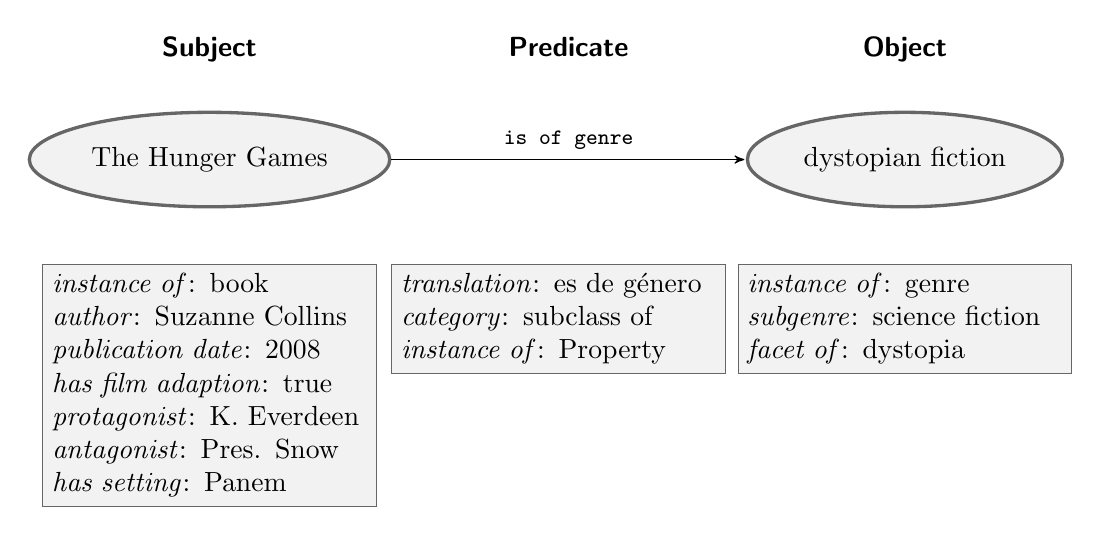
\begin{tikzpicture}[
        vertex/.style={
                ellipse,
                draw=black!60,
                fill=black!5,
                very thick,
                minimum width = 4cm,
                minimum height = 1.2cm
            },
        predicate/.style = {font=\footnotesize\ttfamily},
        >= stealth',
        shorten >= 0.5pt
    ]
    \node[vertex,label={[yshift=0.5cm,font=\sffamily\bfseries]Subject}] (thg) {The Hunger Games};
    \node[vertex,label={[yshift=0.5cm,font=\sffamily\bfseries]Object}] (dystopian) [right=4.5cm of thg] {dystopian fiction};

    \node[draw=black!60,fill=black!5,text width=4cm] (thg_text) [below=0.7cm of thg] {
        \textit{instance of}: book\\
        \textit{author}: Suzanne Collins\\
        \textit{publication date}: 2008\\
        \textit{has film adaption}: true\\
        \textit{protagonist}: K. Everdeen\\
        \textit{antagonist}: Pres. Snow\\
        \textit{has setting}: Panem
    };
    \node[draw=black!60,fill=black!5,text width=4cm] (dystopian_text) [below=0.7cm of dystopian] {
        \textit{instance of}: genre\\
        \textit{subgenre}: science fiction\\
        \textit{facet of}: dystopia\
    };
    \node[draw=black!60,fill=black!5,text width=4cm] (predicate_text) [left=0.15cm of dystopian_text] {
        \textit{translation}: es de género\\
        \textit{category}: subclass of\\
        \textit{instance of}: Property\\
    };

    \path[->] (thg) edge node[predicate,above,label={[yshift=0.7cm,font=\sffamily\bfseries]Predicate}] {is of genre} (dystopian);
\end{tikzpicture}
\end{document}